
\section{Image Generation}
\begin{figure}[htbp]
    \centering
    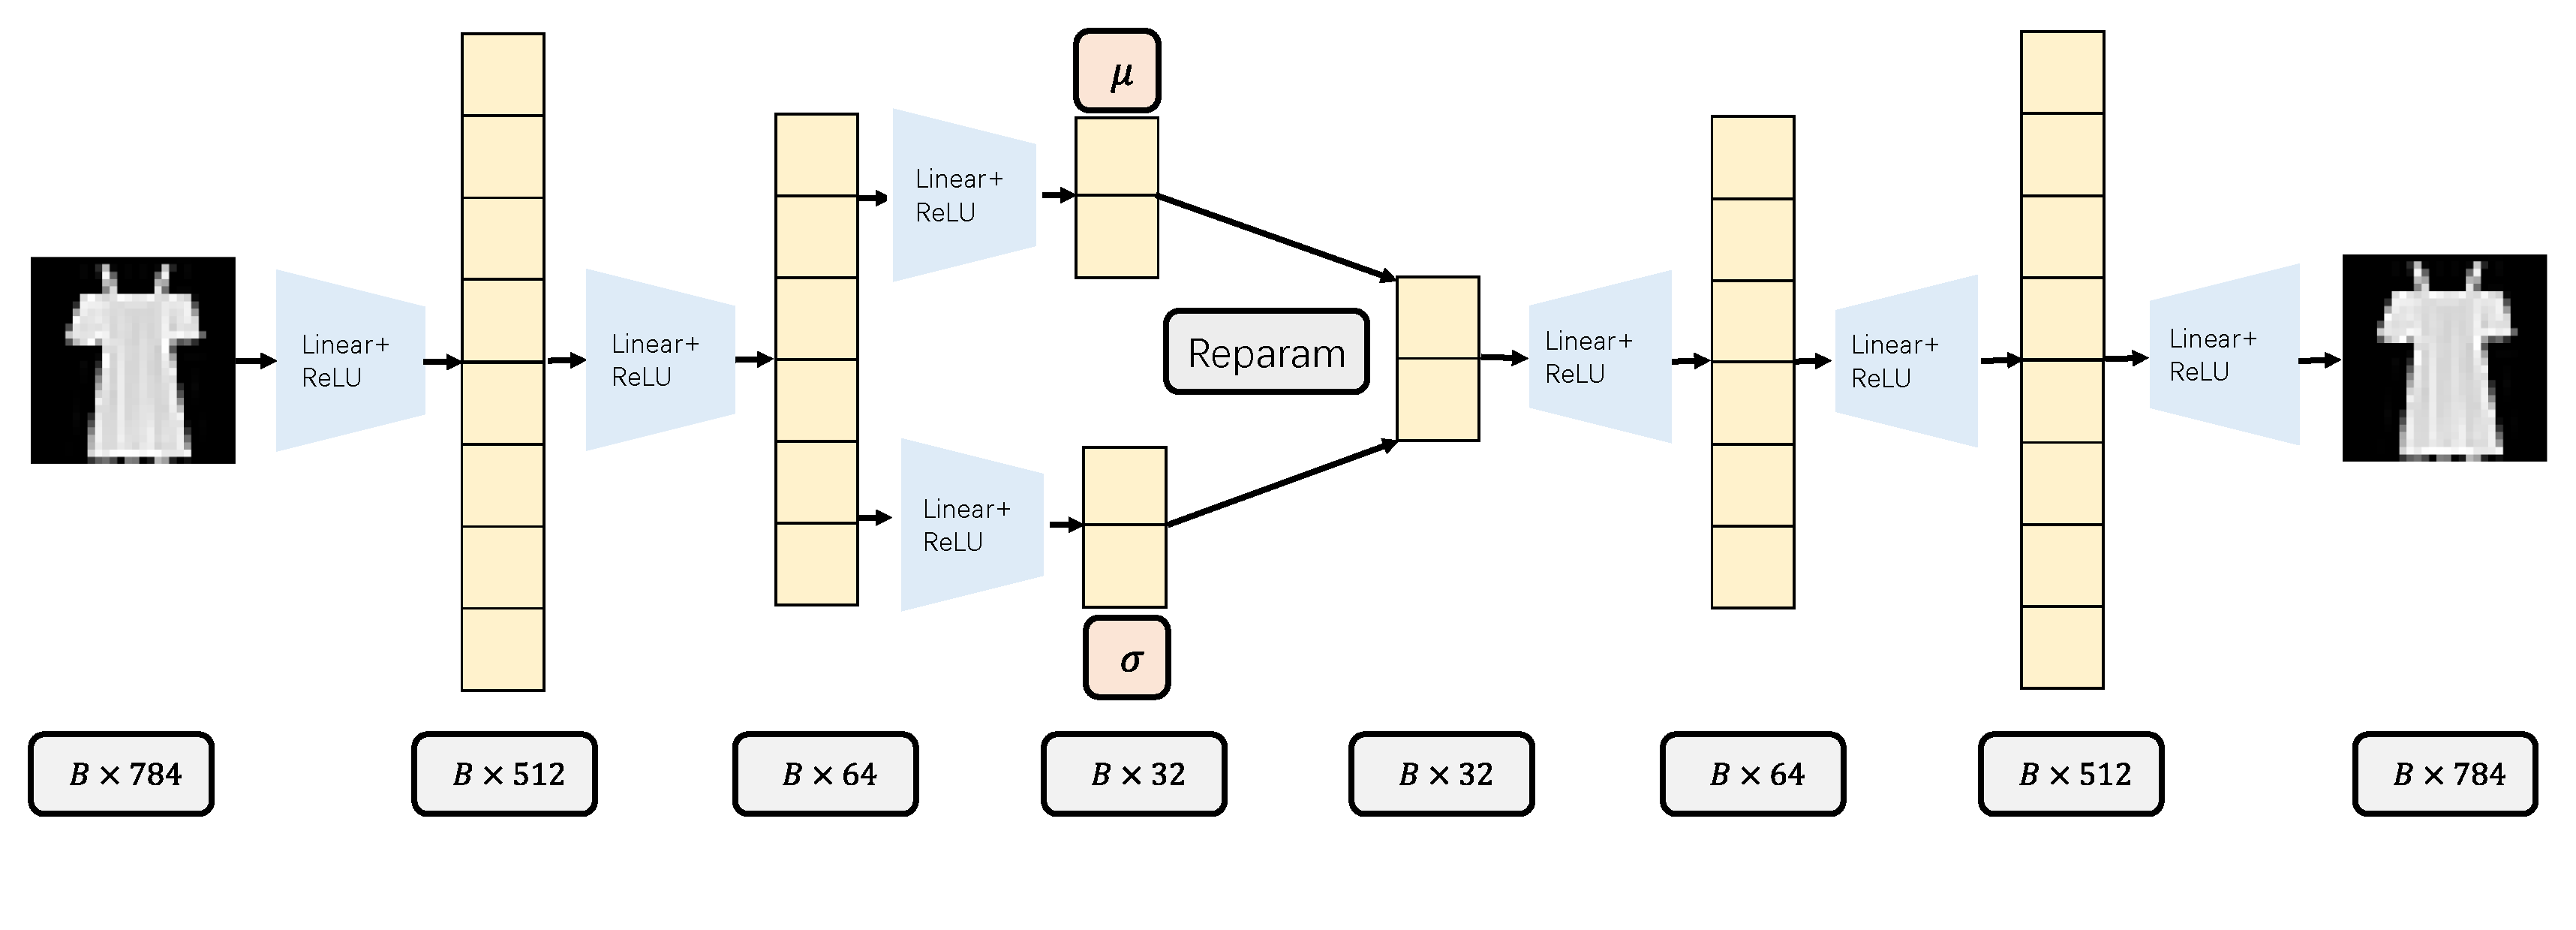
\includegraphics[width=0.95\textwidth]{vae_model.pdf}
    \caption{VAE model framework. }
    \label{fig:vae_model}
\end{figure}
\subsection{Model \& Hyperparameters}
Two different datasets are provided and what I have chosen is FashionMnist dataset, which contains 70000 images with 10 different classes. 
I use 60000 images as the training set and train my VAE model on it.
For evaluation, I randomly initialize two Gaussian noise and use the trained decoder and specified $\alpha$ value to separately output the generated images.
\newline
\newline
\noindent 
I ran my VAE model for 50 epochs.
The batch size is set to 256 for better generalization.
The learning rate is again set to $0.001$.
The detailed model is presented in Fig.~\ref{fig:vae_model}.
In encoder, I use two linear models and respectively learn the expectation and variance of latent normal distribution.
Because outputs of neural networks are not controllable, I choose to learn the logarithm value of variance instead of directly learning variance.
To obtain the variance, the only thing to do is to execute exponential operation, which is convenient and fast.
To obtain the encoded Gaussian noise, the reparameterization is required and shown on below:
\begin{equation}
    \boldsymbol{p} = \mu + \mathrm{exp}(\log(\sigma ^2) / 2)\cdot \boldsymbol{q}
\end{equation}
where $\boldsymbol{q}$ is a Gaussian noise and $\mu$ is the predicted expectation and $\sigma$ is the predicted standard deviation. 
I omit two implementation steps in input stage and output state, where I flatten the image to a 1D array.

\begin{figure}[htbp]
    \centering
    \begin{subfigure}
        \centering
        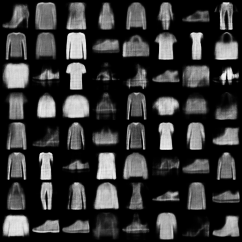
\includegraphics[width=0.45\linewidth]{../images/vae-image1.png}
        % \caption{a}
        \label{fig:vae_image1}
    \end{subfigure}
    % \hfill 
    \begin{subfigure}
        \centering
        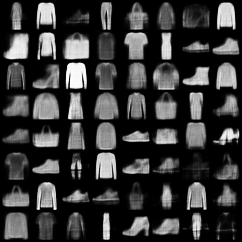
\includegraphics[width=0.45\linewidth]{../images/vae-image2.png}
        % \caption{Absolute value of indivisual components of weight in ridge regression when setting $\lambda$ to 1.0.}
        \label{fig:vae_image2}
    \end{subfigure}
    
    \caption{Two groups of images generated by two batches of random Gaussian noise.}
    \label{fig:vae_original_image}
\end{figure}

\begin{figure}[htbp]
    \centering
    \begin{subfigure}
        \centering
        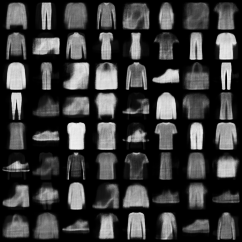
\includegraphics[width=0.32\linewidth]{../images/vae-0.10-merge.png}
        % \caption{a}
        \label{fig:vae_0.1}
    \end{subfigure}
    % \hfill 
    \begin{subfigure}
        \centering
        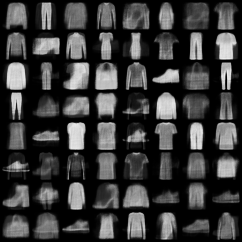
\includegraphics[width=0.32\linewidth]{../images/vae-0.20-merge.png}
        % \caption{Absolute value of indivisual components of weight in ridge regression when setting $\lambda$ to 1.0.}
        \label{fig:vae_0.2}
    \end{subfigure}
    \begin{subfigure}
        \centering
        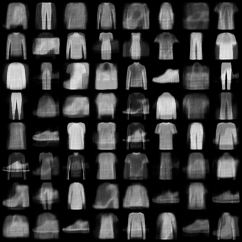
\includegraphics[width=0.32\linewidth]{../images/vae-0.30-merge.png}
        % \caption{Absolute value of indivisual components of weight in ridge regression when setting $\lambda$ to 1.0.}
        \label{fig:vae_0.3}
    \end{subfigure}
    \begin{subfigure}
        \centering
        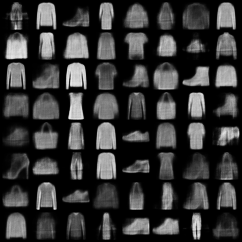
\includegraphics[width=0.32\linewidth]{../images/vae-0.40-merge.png}
        % \caption{Absolute value of indivisual components of weight in ridge regression when setting $\lambda$ to 1.0.}
        \label{fig:vae_0.4}
    \end{subfigure}
    \begin{subfigure}
        \centering
        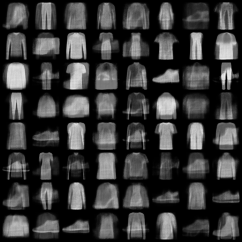
\includegraphics[width=0.32\linewidth]{../images/vae-0.50-merge.png}
        % \caption{Absolute value of indivisual components of weight in ridge regression when setting $\lambda$ to 1.0.}
        \label{fig:vae_0.5}
    \end{subfigure}
    \begin{subfigure}
        \centering
        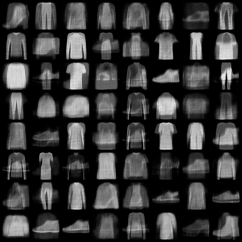
\includegraphics[width=0.32\linewidth]{../images/vae-0.60-merge.png}
        % \caption{Absolute value of indivisual components of weight in ridge regression when setting $\lambda$ to 1.0.}
        \label{fig:vae_0.6}
    \end{subfigure}
    \begin{subfigure}
        \centering
        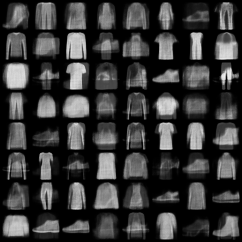
\includegraphics[width=0.32\linewidth]{../images/vae-0.70-merge.png}
        % \caption{Absolute value of indivisual components of weight in ridge regression when setting $\lambda$ to 1.0.}
        \label{fig:vae_0.7}
    \end{subfigure}
    \begin{subfigure}
        \centering
        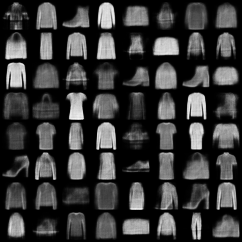
\includegraphics[width=0.32\linewidth]{../images/vae-0.80-merge.png}
        % \caption{Absolute value of indivisual components of weight in ridge regression when setting $\lambda$ to 1.0.}
        \label{fig:vae_0.8}
    \end{subfigure}
    \begin{subfigure}
        \centering
        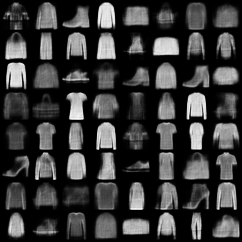
\includegraphics[width=0.32\linewidth]{../images/vae-0.90-merge.png}
        % \caption{Absolute value of indivisual components of weight in ridge regression when setting $\lambda$ to 1.0.}
        \label{fig:vae_0.9}
    \end{subfigure}
    
    \caption{These nine images represent different interpolation values $\alpha$. $\alpha$ values change from 0.1 to 0.9 from left top to right down.}
    \label{fig:vae_samples}
\end{figure}
\subsection{Experiment Result}
I first present two images generated from two random Gaussian noise in Fig.~\ref{fig:vae_original_image}. 
I display 64 different small images generated from a batch for each whole image.
For these two Gaussian noise $\boldsymbol{p}$ and $\boldsymbol{q}$ and use different $\alpha$ values to produce a new image as such:
\begin{align*}
    \mathbf{X}&=\texttt{VAE}(\boldsymbol{p}) \\
    \mathbf{Y}&=\texttt{VAE}(\boldsymbol{q}) \\
    \mathbf{Z}&=\texttt{VAE}(\alpha \boldsymbol{p}+(1-\alpha)\boldsymbol{q})
\end{align*}
where $\mathbf{X,Y,Z}$ represent the generated images and several different examples of $\mathbf{X}$ and $\mathbf{Y}$ are shown in Fig.~\ref{fig:vae_original_image}. 
These nine images represent how a image is transferred from one type of object to another type with different interpolation factors.
Let's look at the first images located at the first row and fourth column in two images in Fig.~\ref{fig:vae_original_image}, which are a T-shirt and a pair of pants, respectively.
Now the $\alpha$ changes from 0.1 to 0.9, which means that the image will transfer from a pair of pants to a T-shirt gradually.
And the images in Fig.~\ref{fig:vae_samples} verify the theoretical results. 
The VAE model implemented by myself can to some extent realize variational image generation.

\subsection{Discussion}
A random Gaussian noise can represent a specific property that the model has learned. But the images generated from VAE may vary according to different noise, which shows the strong variability of VAE models compared to GAN-related models. 
Although GAN models can generate images extremely similar to the original images, they lose the ability to generate diverse images, which is the strength of VAE models.